% CAP description for Tree --> Expand by Indexpath --> Indexpath
\begin{itemize}
\item Use this parameter to specify the indexpath of the subtree you want to expand.
\item Start at the top of the tree. The first node is \bxshell{1}, the second \bxshell{2} etc.
\item Use slash {\tt '/'} as a path separator (to separate parent nodes from child nodes).
\item For example, the second node within the first node is \bxshell{1/2}. 
\item Give the whole path to the node which you want to expand.
\end{itemize}

\textbf{Example:}

\begin{itemize}
\item Your tree looks like this:

\begin{figure}
\begin{center}

\includegraphics{PS/Treeexample3}
\caption{Tree 3}
\label{treeexample3}
\end{center}
\end{figure}

\item You want to expand the tree to node A
\item Enter \bxshell{1/1}:

\begin{figure}
\begin{center}
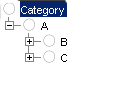
\includegraphics{PS/Treeexample4}
\caption{Tree 4}
\label{treeexample4}
\end{center}
\end{figure}
\end{itemize}
